\documentclass[sigplan,10pt,twocolumn,letterpaper]{article}
%\settopmatter{printfolios=true}
\special{papersize=8.5in,11in}
\setlength{\pdfpagewidth}{8.5in}
\setlength{\pdfpageheight}{11in}
\usepackage[noheadfoot,
            left=1in,right=1in,top=1in,bottom=1in,
            columnsep=0.25in
            ]{geometry}
\usepackage[small,compact]{titlesec}
\usepackage[font={small,bf}]{caption}
\usepackage[nolineno,noindent,norules]{lgrind}
\usepackage{tightenum}
\usepackage{float}
\usepackage{xspace}
\usepackage{times,pifont}
\usepackage{mathptmx}
\usepackage{subfig,graphics,graphicx,color}
\usepackage{multirow}
\usepackage{dblfloatfix} %% correctly orders single- and double-col figures
\usepackage{hyphenat}
\usepackage{mathrsfs}
\usepackage{subfig}
\usepackage{amssymb,amsmath,centernot}
\usepackage{lastpage}
\usepackage{flushend}
\usepackage{hhline}
\usepackage{authblk}
\usepackage[hyphens]{url}
%\newcommand{\doi}{XXXXXX}


%%% ================= START of SOSP '13 template ================= 
% \makeatletter
% 
% \def\ftype@copyrightbox{8}
% \def\@copyrightspace{
% \@float{copyrightbox}[b]
% \begin{center}
% \setlength{\unitlength}{1pc}
% \begin{picture}(20,6.0) 
% \put(0,3){\parbox{\columnwidth}{\scriptsize
% 
% %*** SAMPLE. AUTHOR PUT SUPPLIED TEXT HERE ****
% 
% \noindent
% \rule{6.0 cm}{0.2pt}\\
% Permissiondddd to make digital or hard copies of part or all of this work 
% for personal or classroom use is granted without fee provided that
% copies are not made or distributed for profit or commercial advantage 
% and that copies bear this notice and the full citation on the first
% page. Copyrights for third-party components of this work must be
% honored.  For all other uses, contact the Owner/Author. 
% 
% \vspace{\baselineskip}\noindent
% Copyright is held by the Owner/Author(s).\\
% \textit{SOSP'15}.\\
% ACM XXXXXXX.
% 
% \noindent
% http://dx.doi.org/\doi}
% }
% \end{picture}
% \end{center}
% \end@float}
% 
% \def\maketitle{\par
%  \begingroup
%    \def\thefootnote{\fnsymbol{footnote}}
%    \def\@makefnmark{\hbox
%        to 0pt{$^{\@thefnmark}$\hss}}
%      \twocolumn[\@maketitle]
% \@thanks
%  \endgroup
%  \setcounter{footnote}{0}
%  \let\maketitle\relax
%  \let\@maketitle\relax
%  \gdef\@thanks{}\gdef\@author{}\gdef\@title{}\gdef\@subtitle{}\let\thanks\relax
%  \@copyrightspace}
% 
% \makeatother

%%% ================= END of SOSP '13 template ================= 



%\newcommand{\comment}[1]{}
\frenchspacing
%\doublespacing
%%%%%%%%%%%%%%%%%%%%%%%%%%%%
%     macro

\newcommand{\xxx}{\mbox{\textsc{XXXXX}}\xspace}
\newcommand{\wechat}{\mbox{\textsc{XXXXXX}}\xspace}
\newcommand{\mytitle}[0]{\textbf {Paper Title}}

\newcommand{\mykeywords}[0]{Performance debug}

%%%%%%%%%%%%%%%%%%%%%%%%%%%%%%%%%%%%%%%%%%%%%%%%%%%%%%%%%%%%%%%%%
% hyperref stuff

\usepackage[square,comma,numbers,sort]{natbib}
\usepackage{hypernat}
\usepackage[draft]{hyperref}
%\usepackage{hyperref}

%% fill in pdf info here
\hypersetup{%
colorlinks=false,
pdfborder={0 0 0},
pdftitle={\mytitle},
pdfkeywords={\mykeywords},
bookmarksnumbered,
pdfstartview={FitH},
urlcolor=cyan,
pdfpagelabels=true,
pdfdisplaydoctitle=true,
}%

%\usepackage{breakurl}
%\usepackage[all]{hypcap}
%\renewcommand{\url}{\burl}

%%%%%%%%%%%%%%%%%%%%%%%%%%%%%%%%%%%%%%%%%%%%%%%%%%%%%%%%%%%%
% Some NICE fonts

\newfont{\BIG}{cminch}                             %--- One-inch font
\newfont{\sfbHuge}{cmssbx10 scaled\magstep5}       %-- 25pt sans serif bold
\newfont{\sfbLarger}{cmssbx10 scaled\magstep3}   %-- 12+pt sans serif boldd
\newfont{\sfblarger}{cmssbx10 scaled\magstep2}   %-- 12+pt sans serif bold
\newfont{\sfblarge}{cmssbx10 scaled\magstep1}      %-- 12pt sans serif bold
\newfont{\sfbeleven}{cmssbx10 scaled\magstephalf}  %-- 11pt sans serif bold
\newfont{\sfb}{cmssbx10}                           %-- 10pt sans serif bold
\newfont{\sfeight}{cmss8}                          %-- 8pt sans serif

%%%%%%%%%%%%%%%%%%%%%%%%
%   space tweaking

%\textwidth = 6.5 in
%\textheight = 9.0 in
%\setlength{\topmargin}{-.5in}

%\headheight = 0.0 in
%\headsep = 0.0 in
%\parskip = 0.2in
%\parindent = 0.0in

\renewcommand{\topfraction}{0.95}
\addtolength{\textfloatsep}{-0.1in}
%\addtolength{\floatsep}{0.025in}
\renewcommand\floatpagefraction{.9}
%\renewcommand\bottomfraction{.9}
\renewcommand\textfraction{.1}
%\renewcommand\footnotetextcopyrightpermission[1]{}

\setlength{\parindent}{9pt}

% Rescue
\makeatletter
\def\v#1{{\mbox{\fontfamily{cmtt}\fontsize{\f@size}{\f@size}\selectfont #1}}}

\newcommand{\messaging}[0]{\textsc{Messaging}\xspace}
\newcommand{\pthread}[0]{\mbox{Pthreads}\xspace}

% In short.
\newcommand{\eg}{{e.g. }}
\newcommand{\ie}{{i.e. }}
\newcommand{\etc}{{etc}}
\newcommand{\para}[1]{\vspace{.00in}\noindent{\bf #1}}
\newcommand{\wrt}{{w.r.t. }}
\newcommand{\cf}{{cf. }}
\newcommand{\etal}{{et al. }}

% operations.
\newcommand{\psynchcvwait}[0]{\v{psynch\_cv\_wait()}\xspace}
\newcommand{\send}[0]{\v{send()}\xspace}
\newcommand{\recv}[0]{\v{recv()}\xspace}

% stats.
\newcommand{\proxy}{\mbox{\textsc{Proxy}}\xspace}
\newcommand{\serviceA}{\mbox{\textsc{Service A}}\xspace}

\def\LGfsize{\footnotesize}
%\pagestyle{empty}

\begin{document}

% Hack for: Package caption Error: No float type 'copyrightbox' defined.
%\newcounter{copyrightbox}

\date{}

\title{\mytitle\\
\rm \Large Title For Paper}

\author[+]{\hspace{0 mm}\fontsize{10}{10}\selectfont SOSP
2019 submission \#XX}
\maketitle

\begin{sloppypar}
\begin{abstract}
%Althought many efforts are made to eliminate performance bugs,
%optimizations in both software and hardware,
%they still exist every computing platforms. 
%Spinning beachball is an indicator used to imply performance bugs in Mac.
%However, debugging in such cases are still hard.
%The user should know where the app gets stuck and what exactly causes the hanging(root cause).
%Using lldb to reproduce such bug is impossible due to the high latency caused by the tool.
%It hard to tell if the showing beach ball indicates a performance bug or not.
%Moreover, multiple processing and multiple threading are common used in current system.
%The root cause of the hanging is not straitforward.
%The long latency in the UI thread may caused by a worker thread in the App, event due to the wait on daemons. 
%We proposed XXX which leverage the trace tool by Apple to monitor system wide events 24X7.
%After collecting the data we analyze and tell the user where the stuck redides.
%With the confined range, XXX also provide tools to further execute a conditional debugging.

\end{abstract}
\end{sloppypar}

%%%%%%%%%%%%%%%%%%%%%%%%%%%%%%%%%%%
% Add page number.
\setcounter{page}{1}
\pagenumbering{arabic}

\thispagestyle{plain}
\pagestyle{plain}
\setlength{\footskip}{20pt}
%%%%%%%%%%%%%%%%%%%%%%%%%%%%%%%%%%%

\begin{sloppypar}

\section{Introduction} \label{sec:intro}

Today's web and desktop applications are predominantly parallel or
distributed, making performance issues in them extremely difficult to
diagnose because the handling of an external request is often spread across
many threads, processes, and asynchronous contexts instead of in one
sequential execution segment~\cite{harter2012file}. To manually reconstruct
a graph of execution segments for debugging, developers have to sift
through a massive amount of log entries and potentially code of related
application components~\cite{chen2002pinpoint, zhao2016non, xu2009detecting,
nagaraj2012structured, yuan2012conservative}. More often than not, developers
give up and resort to guessing the root cause, producing ``fixes'' that
sometimes make the matter worse. For instance, a bug in the Chrome browser
engine causes a spinning cursor in macOS when a user switches the input
method~\cite{chromiumbugreport}, was first reported in 2012. Developers
attempted to add timeouts to work around the issue. Unfortunately, the bug has
remained open for seven years and the timeouts obscured diagnosis further.

Prior work proposed what we call \emph{Causal tracing}, a powerful technique
to construct request graphs automatically~\cite{reynolds2006pip, fonseca2007x,
benjamin2010dapper, zhang2013panappticon, ravindranath2012appinsight}. It
does so by inferring (1) the beginning and ending boundaries of the execution
segments (vertices in the graph) involved in handling a request; and (2) the
causality between the segments (edges)---how a segment causes others to do
additional handling of the request. Compared to debuggers such as \spindump that
capture only the current system state, causal tracing is effective at aiding
developers to understand complex causal behaviors and pinpoint the root causes
for real-world performance issues.

Prior causal tracing systems all assume certain programming idioms to automate
inference. For instance, if a segment sends a message, signals a condition
variable, or posts a task to a work queue, it wakes up additional execution
segment. Prior systems assume that wake-ups reflect causality. Similarly, they
assume that the execution segment, from the beginning of a callback invocation
to the end, is entirely for handling related work in a request. Unfortunately,
based on our study and experience of building a causal tracing system for macOS,
we find that modern applications violate these assumptions. Hence, the request
graphs computed by causal tracing are inaccurate in several ways.

First, an inferred segment can be larger than the actual event handling segment
due to batch processing. Specifically, for performance, an application or its
underlying frameworks may bundle together work on behalf of multiple requests
with no clear distinguishing boundaries. For instance, WindowServer in macOS
sends a reply for a previous request and receives a message for the current
request using one system call \vv{mach\_msg\_overwrite\_trap}, presumably to
reduce user-kernel crossings. Second, the graphs can miss numerous causal
edges. For instance, consider data dependencies in which the code sets a flag
(\eg, ``\vv{need\_display} = 1'' in macOS animation rendering) and later
queries the flag to process a request further. This pattern is broader than
ad hoc synchronization~\cite{xiong2010ad} because data dependency occurs
even within a single thread (such as the buffer holding the reply in the
preceding WindowServer example). Although the number of these flags may be
small, they often express critical causality, and not tracing them would lead
to many missing edges in the request graph. However, without knowing where
the flags reside in memory, a tool would have to trace all memory operations,
incurring prohibitive overhead and adding many superfluous edges to the request
graph. Third, inferred edges can be superfluous because wake-ups do not
necessarily reflect causality. Consider an \vv{unlock()} operation waking up an
thread waiting in \vv{lock()}. This wake-up can just be happenstance and the
developer's intent is mutual exclusion. However, the two operations can also
enforce a causal order.

We believe that, without fully understanding of application semantics, request
graphs computed by causal tracing are \emph{inherently} inaccurate and both
over- and under-approximate reality. Although developer annotations can help
improve accuracy~\cite{reynolds2006pip, fonseca2007x}, modern applications use
more and more third-party libraries, whose source code is not available. Given
the frequent use of custom synchronizations, work queues, and data flags in
modern applications, it is hopeless to count on manual annotations to ensure
accurate capture of request graphs.

In this work, we present \xxx, a dramatically different approach in the design
space of causal tracing. It is desgined for tech-savvy users who are intersted
in compiling useful bug reports for their daily use applications, whose source
codes are often not available. As opposed to full manual schema upfront for
all involved applications and daemons~\cite{barham2004using, reynolds2006pip,
fonseca2007x}, \xxx calculates an event graph for a duration of the system
execution with both true causal edges and weak ones, and enables users to
provide necessary schematic information on demand in diagnosis. Specifically, it
keeps humans in the loop, as a debugger should rightly do. \xxx queries users a
judicially few times to (1) resolve a few inaccurate edges that represent false
dependencies and (2) identify potential dependency due to data flags.

We implement \xxx in macOS, which is closed-source on its frameworks and many
applications. This closed-srouce environment therefore provides a true test
of \xxx. We address multiple nuances of macOS that complicate causal tracing,
and build a system-wide, low-overhead, always-on tracer. \xxx enables users to
optionally increase the granularity of tracing (\eg, logging call stacks and
instruction streams) by integrating with existing debuggers such as \vv{lldb}.

We evaluate \xxx on \nbug real-world, open spinning-cursor issues in widely
used applications such as Chromium browser engine and macOS System Preferences,
Installer, and Notes. The root causes of all \nbug issues were previously
unknown to us and, to a large extent, the public. Our results show that \xxx is
effective: it helps us non-developers of the applications find all root causes
of the issues, including the Chromium issue that remained open for seven years.
\xxx mostly needs only less than 3 user queries per issue but they are crucial
in aiding diagnosis. \xxx is also lightweight: its systems-wide tracing incurs
only \cpuoverhead CPU overhead overall.

%% consider adding comparison to prior approaches
%% Our techniques effectively removed false and added missing edges in the
%% event graph.  Even with our techniques, the resultant graph remain too
%% inaccurate for traditional causal tracing, but, fortunately, an average
%% of XXX user queries suffice to locate the root causes accurately.

We make the following contributions: 
\begin{enumerate}

\item We demonstrate conceptual realization that causal tracing is inherently
inaccurate, and introduce interactive approach in the design space of causal 
tracing.

\item We build \xxx, performing system-wide tracing in macOS with little
overhead, and handle several macOS trickeries that complicate causal tracing.

\item We use \xxx to diagnose real-world spinning cursors and find root causes for
performance issues that have remained open for years.

\end{enumerate}

This paper is organized as follows. In Section~\ref{sec:background}, we
introduce the causal tracing and prior works. In Section~\ref{sec:overview},
we present an overview of using \xxx and a Chromium example. In
Section ~\ref{sec:inaccuracy}, we report inherently inaccuracy
patterns observed in macOS , and Section~\ref{sec:implementation}
describes our tracing implementation and tools for user interaction.
Section~\ref{sec:eval} demonstrates the methodology and results from case
studies, as well as performance evaluation. We summarize related work
in Section~\ref{sec:related-work}, and end with conclusion in Section
~\ref{sec:conclusion}.

\section{Background: Casual Tracing} \label{sec:background}

\begin{figure}[tb]
	\footnotesize
    \centering
	 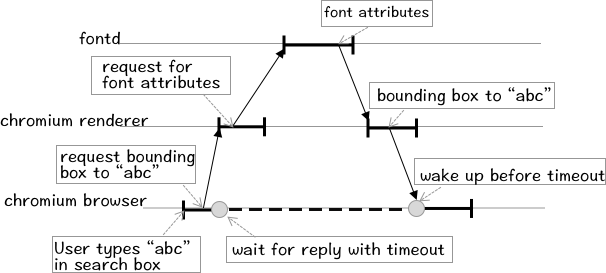
\includegraphics[width=\columnwidth]{./figures/causaltracing_example.png}
    \caption{Handling User Typing in Chromium.  The \vv{browser} and
      \vv{render} each split the work among a main thread and a worker
      thread.  Front service daemon \vv{fontd} uses thread pooling.  For
      clarity, only processes are shown, not their threads.}
    \label{fig:chromium-normal}
\end{figure}

Modern applications are often highly concurrent, spreading the handling of
an external request in multiple threads, processes, and asynchronous
contexts, each of which may multiplex on different requests.  Causal
tracing thus aims to reconnect the execution segments physically separated
in different execution contexts but logically on behalf of the same
request.  Figure~\ref{fig:chromium-normal} shows an example in Chromium,
an open-source browser engine that powers Google Chrome and, starting
recently, Microsoft Edge~\cite{chromiumurl}. When a user types a string in
Chromium, the \vv{browser} process sends an IPC message to the \vv{render}
process where the rendering view and WebKit code run, to calculate the
bounding box of the string.  \vv{render} then queries \v{fontd}, the font
service daemon, to calculate the height and length of the string in the
given font.  Once \vv{fontd} finishes, it sends an IPC reply to wake up
\vv{render} which in turn wakes up \vv{browser}.  The handling of user
typing is thus split among at least three processes and their relevant
threads, and an ideal causal tracing tool would capture these segments
(vertices) and their connections (edges) into a generalized control-flow
graph to aid developer reasoning.

Compared to tools such as \spindump that capture only the current system
state such as the call stack snapshots of each thread, causal tracing
captures the dependency path of events, enabling users to trace across
threads and processes to past events.  For instance, if \vv{render}'s
reply hangs \vv{browser}, causal tracing would enable a developer to
examine \vv{fontd}'s reply to \vv{render}, whereas the \vv{fontd} call
stack that \spindump captures at the time of the hang may be for a
completely irrelevant request.

Mechanically, to build an event graph, causal tracing tools must infer the
beginning and ending boundaries of execution segments and connect a
segment with the other segments that it creates or wakes up. Lacking
application semantics, existing tools make various assumptions to infer
segment boundaries and connections.  We select AppInsight and Panappticon,
two tools closely related to \xxx, and describe how they do so.

AppInsight is designed to help developers understand the performance
bottlenecks in mobile applications.  To infer execution segment
boundaries, it interposes on the interface between the application and
framework, and assumes that the application follows mostly the event
callback programming idiom.  The entry and exit of a callback invocation
delimit an execution segment.  If this segment installs additional
callbacks or signals a waiting thread, then AppInsight connects the
corresponding segments.

Panappticon detects performance issues in Android applications. It traces
low-level events in the Android system and libraries.  To infer execution
segment boundaries and connections, it assumes two programming idioms:
work queue and thread pooling.  For work queue, it marks the handling of a
work item as an execution segment, and connects this segment to the
segment that dispatches the work item.  For thread pooling, it marks from
the wakeup of a worker thread to the wait as an execution segment, and
connects this segment to the segment waking up the worker thread.

%% In this section, we illustrate causal tracing and prior work on it. Causal
%% tracing collects events standing for instrucions executed in CPU and generates
%% a graphical representation with traced events as vertices. Two events always
%% following a sequential constraint reflects causality, which is represented
%% as an edge. The graph helps users understand the complex causal behaviors across
%% thread/process boundaries and attribute bugs to their root causes. Prior works
%% have different definitions of vertices, edges, and root causes based on what
%% events are collected.

%% AppInsight instruments all the upcalls from the framework to the application.
%% It traces user input, display update, the begin and end of procedual call, the
%% invocation of callback function, exception and blocking events in threads. Each
%% event is reflected as a vertex in the request graph. Therefore, the request
%% graph connects (1)user input event to (2)the beginning of event handler, which
%% in turn connects to (3)the beginning of callback in background threads. The
%% vertices like (2) and (3) will connect to (4)the end of the procedual call
%% or lead to (5 )exception. Besides, they will also connect to (6)blocking for
%% signal, if the execution requires synchronization. The goal of AppInsight is to
%% help developers understand the performance bottlenecks with critical paths or
%% exception paths. It defines the root cause as the state of a function execution,
%% long blocking or exception in the application.

%% To be unobtrusive, Panappticon instruments the system to collect low-level
%% and fine grained events from libraries and kernel, including user input,
%% display update, asynchronous call and callback, inter-process comminication,
%% synchronization mechanism, and resource accounting. Every event is a vertex.
%% Panappticon connects continuous vertices which stem from atomic work in a
%% thread, \eg, a worker thread processing one task from a task queue, into an
%% execution interval. Two execution intervals are connected if the earlier
%% interval triggers the latter one. For example, a user input triggering an
%% enqueue message in the same thread reflects as an execution interval, where
%% two vertices are connected with a temperal ordering edge. In another thread,
%% dequeuing the message and submiting an asynchronous task generate another
%% execution interval. The two intervals are connected with a causal edge. With the
%% resouces analysis in every user transaction, from user input to display update,
%% Panapption speculates and manually inspect root causes from design flaws, harmful
%% interaction, to underpowered hardware.

\section{Design}
\label{sec:design}

Our \xxx prototype is designed to debug performance issues in complex modern applications.
It performs lightweight full system tracing of every process including system calls, interprocess messages, and MacOS system daemons.
Offline, we build a graph based on thread executions, with nodes defined by per-event execution segments, and edges wherever there are temporal constraints between threads of execution.

\subsection{Use Cases}

\xxx can be used in two primary ways:
\begin{enumerate}
    \item \xxx can continuously run live in the background and collect full
    system logs. The user works as usual until a crash or performance issue is
    observed.

    \item The user can begin with a reproducible performance issue, and collect
    logs in two situations: a) a baseline situation where the program runs
    normally, and b) a spinning situation that exposes the performance issue.

\end{enumerate}
For a simple issue, like a rare segmentation fault, just having \xxx's lightweight logs may be enough to perform a diagnosis.
However, in most cases, \xxx will need to be used interactively, so the user needs to be able to reproduce the problem.
The user can request more detailed logs in several ways, reproducing the problem, and gathering enough data to narrow in even further on the problem.
The general process for interactive debugging with \xxx is as follows:
\begin{enumerate}
    \item First, the user finds the node \emph{$N_{spin}$} in the \xxx graph
    that corresponds to a hanging thread of execution. The user may leverage
    the system clock time to search for events (\eg, keystrokes).

    \item Next, the user attempts to find the node in the normal case that
    corresponds with $N_{spin}$. There will likely be many possible candidates
    at first, so the user can narrow in on specific nodes and gather more
    detailed information in that area of the program.

    \item Now, with knowledge of $N_{spin}$ and (a small number of) matching
    nodes in the normal graph, the user performs a backward slice through the
    graphs to attempt to find the defining difference between the cases. This
    difference should accurately predict whether a given log represents a
    normal or spinning case, and usually indicates quite directly the root
    cause. As before, additional information may need to be collected from
    certain points in the program to be able to distinguish between the cases.

\end{enumerate}
As shown in Figure XXX, the user's main operations are a) manual inspection of
the graph, b) performing slicing on the graph to show dependent nodes, c)
selecting a graph node to gather more information about, and d) comparing graph
slices between normal and spinning cases.

\section{Implementation}\label{sec:implementation}
We now discuss how we collect tracing events from both kernel and libraries.

\subsection{Event Tracing}

Current MacOS systems support a system-wide tracing infrastructure built by
Apple ~\ref{linktotracetool}. By default, the infrastructure temporarily stores
events in memory and flushes them to screen or disk when an internal buffer is
filled. We extended this infrastructure to support larger-scale tests and avoid
filling up the disk with a file backed ring buffer. Subject to configurarion,
it allows at most 2GB of data per log, which corresponds to approximately
18,560,187 events (about 5 minute with normal operations).

The default tracing points in MacOS do not provide enough information to
generate a dependency graph. As a result, we both patch source code of kernel
and binary instrument libraries to gether more tracing information.

\subsection{Instrumentation}

On MacOS, most libraries as well as many of the applications used day-to-day are
closed-source. To add tracing points to such code, techniques such as library
preloading to override individual functions are not applicable on MacOS, as
libraries use two-level executable namespaces~\cite{}. Hence, we implemented
a binary instrumentation mechanism that allows developers to add tracing at
any location in a binary image. Like Detour~\cite{hunt1999detours}, we use
static analysis to decide which instrumentation to perform, and then enact this
instrumentation at runtime.

%XXX I thought a user can specify a search sequence of instructions, and our
%system adds instrumentation when the sequence is found in binary.  If so we
%want to emphasize it a bit as this feature is different from detour.
%XXX say that instrumentation code is written in C
In \xxx, we patched the kernel with 1193 lines of code, and instrumented
the libraries including: libsystem\_kernel.dylib, libdispatch.dylib,
libpthread.dylib, CoreFoundation, CoreGraphics, HIToolbox, AppKit and QuartzCore,
with our binary instrumentation. 

Now we talk about our instrumentation mechanism. Firstly, users find a location
of interest in the image related to a specific event by searching a sequence of
instructions. Then the users replace a call instruction to invokes a trampoline
target function, in which we overwrite the victimed instructions and produce
tracing data with API from Apple. All of the trampoline functions are grouped
into a new image, as well as an initialization function which carries out the
drop-in replacement. Then command tools from \xxx helps to configure the image
with the following steps: (1)re-export all symbols from the original image so
that the original code can be called Like an shared library; (2)replace the
original image with the new one by renaming them to ensure the modifications
are properly loaded; (3)invoke the initialization function externally through
\texttt{dispatch\_once} during the loading.

%%One potential issue is that we use 5-byte call instructions with 32-bit
%%displacements to jump from the original library to our new one.  This design
%%requires that the libraries be loaded within +/- 2GB of each other in the
%%64-bit process address space.  However, since we list each original library as
%%a dependency of our new libraries, the system loader will map each new and
%%original library in sequence.  In practice, the libraries ended up very close
%%to one another and we did not see the need to implement a more general
%%long-jump mechanism.

%%\subsection{Tracing Custom Primitives} \label{subsec:tcp}
\subsection{User Interaction} \label{subsec:tcp}

%%XXX give a simple command line example of how a user can ask \xxx to trace a
%%data flag
%%XXX say what we do in watch point exception handler (record instruction so
%%can determine read or write, and reg values)

As described in (\S\ref{subsec:userinteraction}), under-connection due to
the missing share data dependency requires users'interaction. \xxx provides
a command line tools to record the share\_flag\_write and share\_flag\_read
events in ad-hoc manner. The tool takes the process id, path to image where the
variable is defined and the symbol of the variable as input. We show the simple
example how a user ask \xxx to trace \_gOutMsgPending in the following command.

\begin{BVerbatim}
./bp_watch pidofWindowServer \
	Path/to/CoreGraphics _gOutMsgPending
\end{BVerbatim}

\xxx hooks the watch point handler in CoreFoundation to make sure that it is
loaded correctly into the address space of our target application. The handler
invokes the event tracing API from Apple to record the value of the shared
variable and the operation type: read or write.

\subsection{Capturing Instructions for Diagnosis}

%XXX Talk about what data we gather using lldb, the debugger in the LLVM compiler tool chain.

After the offline analysis on the graph, we take the API covers the fine range
as input to our debugging scripts.  The debugging scripts go throught the
instruction from application and higher level frameworks step by step.  The
purpose is to capture the parameters results from the user interaction.  Once a
new function begins by checking the instruction, we record the call stacks for
comprehension.  For API from the low level libraries, such as pthread, we step
over and record the return value. The debugging log in this step records the
instruction and its address, callstacks when a \textit{call} instruction is reached,
and return values of \textit{req} instruction. As the operation are confined in the
small range, the overhead is not too much.

Both the execution on normal case and problematic case are recorded, our tool
further compares the log and report the difference, with the full call stack.

%%\subsection{Finding Similar Events}
%%
%%The performance isssue caused by the busy processing in UI thread is quite
%%straightforward to diagnoze with our tool. Debugging the UI thread blocking on
%%the contention of resource is much more difficult.  In this situation, our tool
%%is required to recognize the corresponding node which obtained the resource in
%%its normal execution.
%%
%%Node comparision algorithm helps to allieviate users from the burden of
%%inspecting large logs.  We first normalize the nodes with selected events.  In
%%our system, we exclude the interrupts from the comparison since the number and
%%type of interrupts are usually different from execution to exection.  For the
%%events that connected to other events, we normalize it with a peer attribute to
%%record the process id of its connecting peer, We also record the name of the
%%system calls, message id carried in mach\_msg for corresponding events.  The
%%comparison algorithm omits the repeating times of the same events, by checking
%%if one node contains all distinct events in the other node.
%%
%%The above step only idenfity the similarity of nodes.  We also define the
%%differential attribtes to distinguish the normal node and spinning node,
%%including the waiting time, execution time and system call return values.

\section{Case Studies}
We apply our tools to two realworld bugs.
Both of them are long listed in public.
The chromium bug has been reported multiple times in the chromium bug report.
It is essentially a deadlock bug.
Timeout was added and it turned out a livelock bug.
Cache mechanism is added to alieviate but not solve it ultimately.
The bug of the System Preferences is exposed by an app called DisableMonitor.
Basiclly the app can change some system settings and eventually reveal the inappropriate displayer management
in the Core Graphics.
\subsection{Chromium IME responsive}
One of the long lasting performance issue in chromium is hanging caused by the non-English input.
When users try to type non English to textFields, such as search box,
the main thread of the browser becomes non responsive.
With lldb it is not hard to tell that the main thread get stuck on FindFirstRect,
where the main thread waits for the signal of condition variable.
According to the history in bug report, the developers realized there were deadlocks somewhere.
However, it was hard to pinpoint due to the multiprocess and multithread programing paradigms.
As a result, timeout was added to prevent the deadlock, but not the long latency.
Although a further bug patch introducing cache helps to eliminate the long hanging mostly, 
the performance issue still appears from time to time.
The senario we can reproduce is to open the website of yahoo and quickly type Simplified Chinese.

The ground true we reveal with out tool is as shown in the picture XXX.
In chromium, there are one browser process and multiple renderer processes.
The main thread of the browser process try to get the caret position.
It sends out the message and wait for the reply on a condition variable.
Usually, a worker thread in the browser process will return the firstrect and wake up the main thread.
Howeve, it requires the message from the main thread of a renderer process to proceed.
Without the message from the renderer process, the worker thread is not able to signal the main thread,
thus, the main thread in will always time out.

Our trace tool will collect the data system wide, therefore, all the thread relationships are captured.
With the trace log size, both the hanging case and non-hanging case are recorded.
From the shared condition variable between threads, we are able to align the logs of the two cases,
and discover the missing message in the hanging case.

As we known the unresponsive of the main thread in the renderer process,
we further consult the analyzed trace log and observe that it is waiting on a semaphre,
and eventually waken by the main thread of the browser process.

Our tool further reveal the root cause of the livelock with conditional debugging.
We can either binary instrument or modify the source code to make the renderer thread accept the attachment of lldb.
The concrete call stacks from lldb disclose the task processing in the renderer thread is related to running javascript.

\subsection{System Preferences spin}
System Preferences is the application in MacOS for users to modify various settings.
Displays in the Panel allows user to rearrange the position of displays, but it does not support the disabling of a montor online.
DisableMonitor is an application used to complete the function, easily disabling/enabling  monitors withou unplug them.
Surprisingly, the operation of DisableMonitor exposed a performance bug in System Preferences.
If we disable an external monitor and arrange them afterward, the window System Preferences freezes for seconds.
We enabled Argus on the background and collect the data by normally arranging the displays and reapeating the spinning sequence.

It is not hard to tell the spinning node in the UI thread with our tool.
However, to find the normal node corresponding to the spinning node is not straightforward as in the previous case.
The execution segment includes two types of events: ``\v{mach\_msg}'' and ``\v{thread\_switch}''.
Both of them are used to waiting for the data available ping.
The semantics of the execution segment is not descriptive enough
to identify the normal nodes in the same operation stage.

In the case we detected the intensive timeout in the node,
our search algorithm identify the corresponding normal node by searching the similarity of their proceding nodes.
We find out the path of the normal path as shown in the Figure \ref{fig:path slicing for system preference}.
Our lightweight callstacks were used to verify the correctness of the findings.

The normal node showed it proceeded to \textit{displayReconfigured} after received the message with id 29675.
The spinning node fell into the ``\v{thread\_switch}'' after receiving the message with the same id,
and end up to send message for the available datagram ping with \textit{CGSSnarfAndDispatchDatagrams} again.
The proceding nodes before them sent message to WindowServer for \textit{activeDisplayNotificationHandler}.

With the result, we initiate the concrete debugging by filling the debugging script with the APIs reported.
We set the method \textit{activeDisplayNotificationHandler} as a beakpoint where the script begins debugging.
\textit{displayReconfigured} and \textit{CGSSnarfAndDispatchDatagrams} are recorded to indicate the end of debugging for the normal case and spinning case respectively.

Our debugging scripts ran within the confined range for both the noraml and the spinning execution.
The logs are generated as shown in Figure \ref{fig:step debug log for system preferences}.
By diff the two logs, it is easy for the user to notice the differen braches in \textit{display\_notify\_proc},
which is resulted from its prameter standing for the datagram type.

We make use of the diassembly tool, and reveals the story in the background.
Datagrams from the WindowServer makes applications to handle notifications.
The datagram causes difference are used to finish display reconfiguration for System Preference.
However, in the spinning case the reconfiguration got initiated but not completed.
The main thread leveraged thread\_switch to wait for the flollowing datagram and resulted in a freeze.
As a conclusion, the handler display\_notify\_proc is not appropriately implemented.


\section{Evaluation}
We first presents the results from the live deployment of Argus.
We demonstrate the overhead of our tracing tool intruduced, regarding the storage, memory and CPU usage.
Then we list the softwares which trigger spinning wait cursors in MacOs and the root cause we figure out with our framework.
The list of real-world softwares includes TextEdit, CodEdit, Notes, Hopper Disassembler, Installer, Squel Pro, GetiPlayerAutomator.
At the end, we summaries the tedious work that our tool can take over from the user and make the diagnosis much easier in the wild.

\begin{figure}[tb]
    \centering
    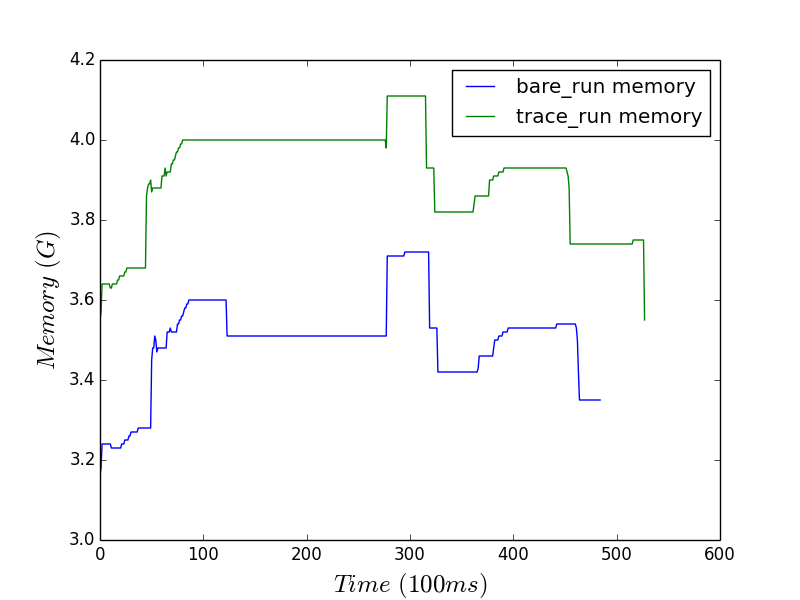
\includegraphics[width=1.0\linewidth]{ibench_memory_compare.png}
    \caption{Memory overhead with tracing.}
    \label{fig:ibench_memory_overhead}
\end{figure}

\begin{figure}[tb]
    \centering
    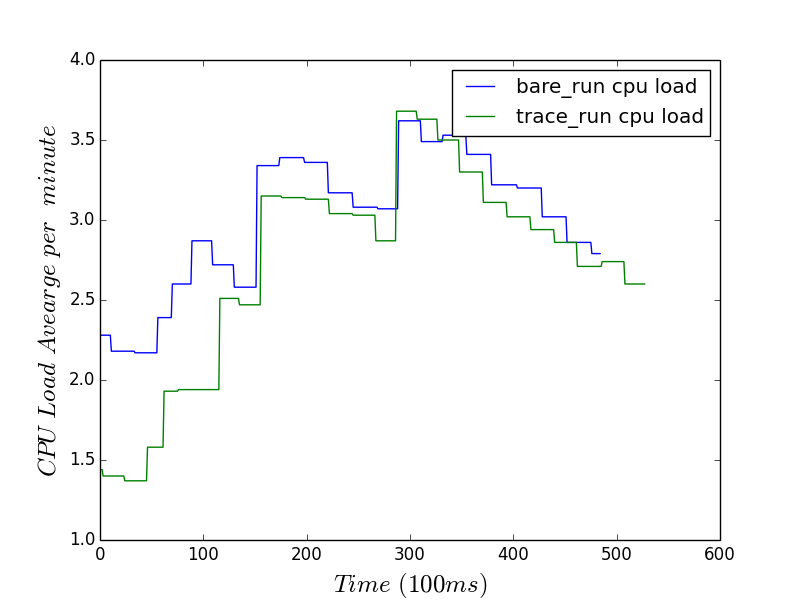
\includegraphics[width=1.0\linewidth]{ibench_cpuload_compare.png}
    \caption{CPU overhead with tracing.}
    \label{fig:ibench_cpu_overhead}
\end{figure}

\begin{itemize}
\item tracing overhead
	\begin{itemize}
	\item memory and CPU usage on top, while running ibench with and without our tracing enabled
	\item memory and CPU usage on top, while running the listed real world applications with and without our tracing enabled
	\item how much times it takes to filled the buffer we fixed 2G
	\item how many events recorded in the buffer
	\end{itemize}
\item number of edges and nodes in the graphs and portions of data the user need to examine to figure out the root cause.
\end{itemize}

\input{discussion}
\section{Related Work}
\label{sec:related-work}

While there is currently no system that can help users debug performance
issues in closed-source applications on proprietary macOS, several active
research topics are closely related.

\para{Event tracing.}
\begin{table}[ht]
\footnotesize
\centering
  \begin{tabularx}{\columnwidth}{l|XXX}
  \hline
Paradigm & Panappticon & AppInsight & \xxx\\
\hline
\hline
%User input & \mycheck & \mycheck & \mycheck \\
%Display update & \mycheck & \mycheck & \mycheck\\
Async calls & MessageQueue, & Upcall & libdispath\\
			& ThreadPoolExecutor &  & runloop \\
			&	&	&timer\\
IPC calls & \mycheck & \mycross & \mycheck \\
Batching & \mycross & \mycross & \mycheck \\
Data flag & \mycross & \mycross  & \mycheck \\
Wait-Wakeup & 4 primitives & Silverlight methods & system wide \\
%Fork & \mycheck & \mycorss & \mycross \\
%Interrupts &\mycross & \mycross &\mycheck\\
%Timeshare Maintain &\mycross &\mycross &\mycheck\\
%Syscall and backtrace
\hline
  \end{tabularx}
  \caption{Programming paradigms tracked.} 
  \label{table:paradigms}
\end{table}


Panappticon \cite{zhang2013panappticon} monitors a mobile system and uses the
trace to characterize the user transactions of mobile apps. Although it aims to
track system-wide events and correlate them without developer input, it supports
only two models of communication: work queue and thread pooling. AppInsight
\cite{ravindranath2012appinsight} instruments application to identify the
critical execution path in a user transaction. It supports the event callback
pattern, and does not trace across process or app boundaries.
Magpie~\cite{barham2004using} monitors server applications in Windows with the
goal to model the normal behaviors of a server application in response to a
workload. This model further helps detecting anomalies statistically. Magpie
requires a manual-written event schema for all involved applications to capture
precise request graphs, whereas \xxx has a simple, application-agnostic schema
for system-wide tracing and enables users to provide more application-specific
knowledge on demand.

Aguilela \cite{aguilera2003performance} uses timing analysis to correlate
messages to recover their input-output relations while treating the application
as a black box. XTrace, Pinpoint and \etc ~\cite{fonseca2007x, chen2002pinpoint,
chow2014mystery} trace the path of a request through a system using a unique
identifier attached to each request and stitch traces together with the
identifier. \xxx comes up violation patterns and does not assume the presence of
a unified identifier in closed-source, third-party applications, frameworks, and
libraries.


\para{Performance anomaly detection.}
Several systems detect performance
anomalies automatically. \cite{han2012performance, yuan2012conservative}
leverage the user logs and call stacks to identify the performance anomaly.
\cite{cohen2004correlating, saidi2008full, xu2009detecting, du2017deeplog}
apply the machine learning method to identify the unusual event sequence as an
anomaly. \cite{yu2014comprehending} generates the wait and waken graph from
sampled call stacks to study a case of performance anomaly.

These systems are orthogonal to \xxx as \xxx's goal is to diagnose an
already-detected performance anomaly. These systems can help \xxx by detecting
more accurately when a performance issue arises.

\section{Conclusion} \label{sec:conclusion}
Our key insight in this paper is that causal tracing is inherently
imprecise. We have reported patterns we observed that pose big precision
challenges to causal tracing, and built \xxx, a practical system for
effectively debugging performance issues in macOS applications despite the
imprecision of causal tracing.  To do so, it lets a user provide domain
knowledge interactively on demand. Our results show that \xxx effectively
helped us locate all root causes of the issues, including a bug in Chromium,
01 and incurred 12\% CPU overhead overall in its system-wide tracing.

\end{sloppypar}

\clearpage
% uncomment to tweak with bib spacing
%\setlength\bibsep{2.25pt}
{
%\small
 \bibliographystyle{abbrvnat}
 \bibliography{bib/biblio}
}

\end{document}
